%#!platex main

\chapter{文脈自由文法}
\label{151253_30Mar06}

構文解析部の処理では、何らかの形で原始プログラム言語の構文をコンピュータ
で扱わなければならない。\ref{175712_30Mar06}章で取り上げた正則表現は、原
始プログラム言語で扱う字句要素を定義することはできるが、それらをどのよう
に組み合わせれば文法的に正しいのか、については定義することができない。

本章では、プログラミング言語の構文を扱うための基本的な理論である文脈自由
文法について説明し、構文解析に必要ないくつかの重要な性質について述べる。

なお、本章でも\ref{175712_30Mar06}章で述べた言語理論に関する用語を用いる。

\section{文脈自由文法}

\subsection{定義}

プログラミング言語の構文を定義するには、通常、{\bfseries 文脈自由文
法}(context free grammar)を用いる。例えばC言語のif文の構文は、
文脈自由文法では次のように書くことができる。
\begin{align*}
 selection\_statement & \rightarrow {\sf if}\ {\sf (}\ expression\ 
  {\sf )}\ statement \\
 selection\_statement & \rightarrow {\sf if}\ {\sf (}\ expression\ 
  {\sf )}\ statement\ 
 {\sf else}\ statement\ 
\end{align*}

矢印$\rightarrow$とその両辺からなる式を{\bfseries 生成規則}(production
rule)、もしくは略して{\bfseries 規則}(rule)という。生成規則の左辺は記
号1つ、右辺は記号列から成っている。記号は{\bfseries 非終端記
号}(nonterminal symbol)と{\bfseries 終端記号}(terminal symbol)に分け
られる。この例では、$selection\_statement$, $expression$, $statement$が非
終端記号、{\sf if}, {\sf (}, {\sf )}, {\sf else}が終端記号である。生成規
則の左辺には非終端記号しか出現できない。右辺には非終端記号、終端記号とも
に出現することができる。非終端記号のうち1つを特に{\bfseries 開始記
号}(start symbol)という。

もう1つ例として「数字、$+$、$-$からなる式」を表す文脈自由文法を示そう。
\begin{equation}
 \begin{split}
 list & \rightarrow list\ {\sf +}\ digit \\
 list & \rightarrow list\ {\sf -}\ digit \\
 list & \rightarrow digit \\
 digit & \rightarrow {\sf 0} \mid {\sf 1} \mid {\sf 2} \mid {\sf 3}
  \mid {\sf 4} \mid {\sf 5} \mid {\sf 6} \mid
  {\sf 7} \mid {\sf 8} \mid {\sf 9}
 \end{split}\label{171007_30Mar06}
\end{equation}

この例では$list$, $digit$が非終端記号、数字と${\sf +}$, ${\sf -}$が終端記
号である。また、最後の規則の$\mid$は「または」の意味である。なお、この例
から分かるように、左辺の非終端記号が同じ生成規則の右辺に出現してもかまわ
ない。

まとめると、文脈自由文法$G$は次のような構成要素からなる。
\begin{enumerate}
 \item 非終端記号の有限集合$V$
 \item 終端記号の有限集合$T$
 \item 生成規則の有限集合$P$
 \item 開始記号$S \in V$。非終端記号のうち1つ
\end{enumerate}

記号を1つも含まない列もある。これを{\bfseries 空列}(empty string)とよび、
$\epsilon$という記号で表す。また、プログラミング言語の構文を表す表現とし
て、ほかに{\bfseries BNF 記法}(Backus Naur Form)というものがあるが、文
脈自由文法とほぼ同じと考えてよい。BNF記法で上の文法を書くと次のようになる。
\begin{align*}
 list & ::= list + digit \\
 list & ::= list - digit \\
 list & ::= digit \\
 digit & ::= 0 \mid 1 \mid 2 \mid 3 \mid 4 \mid 5 \mid 6 \mid 7 \mid 8
 \mid 9 
\end{align*}

% \begin{example}
%  次の文法は、簡単な算術式を定義するものである。
%  \begin{eqnarray*}
%   expr & \rightarrow & expr\ op\ expr \mid (\ expr\ )\mid -\ expr\mid
%    {\bf id} \\
%   op & \rightarrow & + \mid - \mid * \mid / 
%  \end{eqnarray*}$\Box$
% \end{example}

以降の説明では、次のように記法を決めておくことにする。
\begin{enumerate}
 \item 前のほうの英小文字($a, b, c, \cdots$)、演算子記号($+, -, \cdots$)、
       括弧やコンマなどの区切り記号、数字、太字の記号列は終端記号を表す。
 \item 前のほうの英大文字($A, B, C, \cdots$)、$S$ (開始記号)、英小文字の
       イタリック体の名前({\itshape expr}, {\itshape stmt}など)は非終端記
       号を表す。
 \item 後ろのほうの英大文字($X, Y, Z, \cdots$)は非終端記号または終端記号
       を表す。
 \item 後ろのほうの英小文字($w, x, y, z, \cdots$)は終端記号列を表す。
 \item 小文字のギリシャ文字($\alpha, \beta, \gamma, \cdots$)は、記号列(終
       端記号と非終端記号が混ざっていてよい)を表す。
 \item 最初に現れる生成規則の左辺を開始記号とする。また、$S$を開始記号と
       することが多い。
\end{enumerate}

\subsection{文脈自由文法の意味}

文脈自由文法$G = (V, T, P, S)$は、$T$、すなわち終端記号の集合をアルファベッ
トとする言語を表している。では、具体的にどのような言語を表しているのだろ
うか。

文法の言語の定義方法にはいくつかあるが、その1つに「生成規則を書き換え規則
と考える」というものがある。つまり、開始記号$S$を$S$-生成規則の右辺の記号
列$\alpha$で置き換え、さらに$\alpha$に含まれる非終端記号を、その記号の生
成規則の右辺で置き換える。この操作を、記号列が終端記号のみになるまで繰り
返す。このようにして得られる終端記号列すべての集合を、その文法の
{\bfseries 言語}(language)という。

\begin{example}
 \eqref{171007_30Mar06}の文法
 \begin{align}
  list & \rightarrow list\ {\sf +}\ digit\label{171930_30Mar06} \\
  list & \rightarrow list\ {\sf -}\ digit\label{172048_30Mar06} \\
  list & \rightarrow digit\label{172152_30Mar06} \\
  digit & \rightarrow {\sf 0} \mid {\sf 1} \mid {\sf 2} \mid {\sf 3}
  \mid {\sf 4} \mid {\sf 5} \mid {\sf 6} \mid
  {\sf 7} \mid {\sf 8} \mid {\sf 9}\label{172302_30Mar06}
 \end{align}
 について、\eqref{171930_30Mar06}を用いると、開始記号$list$を右辺の記号列
 $list + digit$に置き換えることができる。これを繰り返すと、以下のように終
 端記号列$9-5+2$を得ることができる。
 \begin{align*}
  \underline{list} & \Rightarrow \underline{list} + digit &&
  \text{\eqref{171930_30Mar06}を適用} \\
       & \Rightarrow \underline{list} - digit + digit &&
  \text{\eqref{172048_30Mar06}を適用} \\
       & \Rightarrow \underline{digit} - digit + digit &&
  \text{\eqref{172152_30Mar06}を適用} \\ 
       & \Rightarrow 9 - \underline{digit} + digit && \text{\eqref{172302_30Mar06}を
  適用} \\
       & \Rightarrow 9 - 5 + \underline{digit} && \text{\eqref{172302_30Mar06}を適用} \\
       & \Rightarrow 9 - 5 + 2 && \text{\eqref{172302_30Mar06}を適用}
 \end{align*}
\end{example}

もう少し形式的に書くと次のようになる。生成規則$A \rightarrow \gamma$を記
号列$\alpha A\beta$に適用して$A$を$\gamma$に置き換えると
$\alpha\gamma\beta$となる。このとき、$\alpha A\beta$から
$\alpha\gamma\beta$が{\bfseries 導出される}(derive)といい、$\alpha
A\beta \Rightarrow \alpha\gamma\beta$と表す。$\alpha_1$に0回以上置き換え
を適用して$\alpha_n$が導出されるとき、$\alpha_1
\stackrel{*}{\Rightarrow} \alpha_n$と書く。
$S \stackrel{*}{\Rightarrow} \alpha$のとき、$\alpha$を{\bfseries 文形式}
(sentential form)という。とくに$\alpha$が終端記号のみからなるとき、
{\bfseries 文}(sentence)という。

文法$G$の言語$L(G)$とは、$L(G) = \{w \mid S \stackrel{*}{\Rightarrow}
w\}$である。ただし$S$は$G$の開始記号である。すなわち、$G$の言語とは、
$G$の開始記号から導出される文の集合である。


\section{解析木と導出}

文脈自由文法の開始記号にどのように生成規則が適用され、終端記号列が生成さ
れたのかを図示したものを{\bfseries 解析木}(parse tree)という。解析木は、
導出の様子を図示したものであると考えられ、文の ``構文的な構造''を表したも
のだと言える。例えば、\eqref{171007_30Mar06}に示した文脈自由文法について、
式$9-5+2$の解析木は図\ref{152653_30Mar06}のようになる。

\begin{figure}
 \begin{center}
  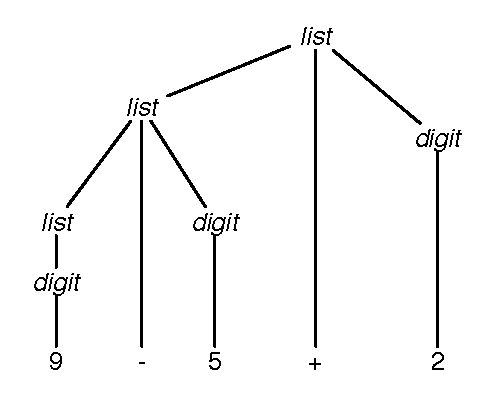
\includegraphics{figure/parse_tree_01.pdf}
 \end{center}
 \caption{解析木の例}
 \label{152653_30Mar06}
\end{figure}

形式的には、解析木は次のような木である。
\begin{enumerate}
 \item 根は開始記号をラベルとして持つ。
 \item 葉は終端記号または$\epsilon$をラベルとして持つ。
 \item 内部の節は非終端記号をラベルとして持つ。
 \item 非終端記号Aをラベルに持つ内部の節の子が左から順に$X_1, X_2,
       \cdots, X_n$とすると、$A \rightarrow X_1 X_2 \cdots X_n$は生成規則
       である。$A \rightarrow \epsilon$に対しては、節$A$は$\epsilon$をラ
       ベルとする子を持つ。
\end{enumerate}

解析木の葉を左から右に読んでいくと、終端記号列が得られる。これが開始記号
から生成される終端記号列、すなわち文である。これを解析木の{\bfseries 結
果}(result)という。

\subsection{解析木の意義}

解析木は、式の値を計算したりプログラムを翻訳する際にいろいろ役立つ。例え
ば、先に述べた数式の値を計算することを考えよう。各非終端記号が属性$v$を持
ち、各生成規則に次のようなプログラム片が付けられているとする。なお、左辺
と右辺に同じ非終端記号が出現する場合には、便宜上、それぞれ$l$と$r$という
添字を付けて区別している。
\begin{align*}
 list & \rightarrow list + digit \quad \{ list_l.v = list_r.v + digit.v; \} \\
 list & \rightarrow list - digit \quad \{ list_l.v = list_r.v - digit.v; \} \\
 list & \rightarrow digit \quad \{ list.v = digit.v; \} \\
 digit & \rightarrow 0	\quad \{ digit.v = 0; \} \\
 digit & \rightarrow 1	\quad \{ digit.v = 1; \} \\
 \cdots \\
 digit & \rightarrow 9 \quad \{ digit.v = 9; \} \\
\end{align*}

解析木の節点の属性$v$の値を、その節点に対応する生成規則に付けられたプログ
ラム片に基づいて計算すると、その解析木の結果である式の値が求められる。式
$9 - 5 + 2$の解析木による例を図\ref{190545_30Mar06}に示す。この計算は、解
析木を深さ優先で探索し、帰りがけにプログラム片を実行することに相当してい
る。

\begin{figure}
 \begin{center}
  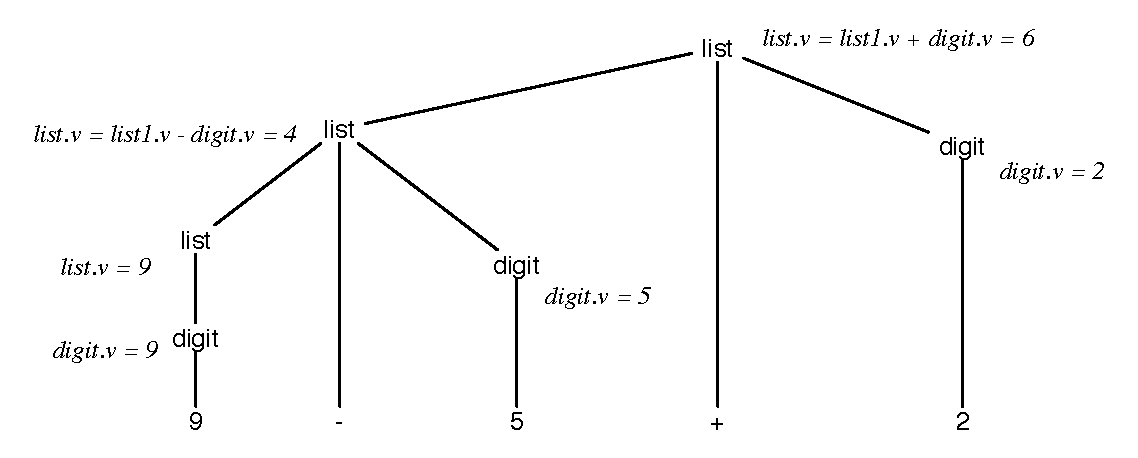
\includegraphics[width=12cm]{figure/parse_tree_appl.pdf}
 \end{center}
 \caption{解析木による式の値の計算}
 \label{190545_30Mar06}
\end{figure}

\section{最左導出、最右導出}

文法$G$の開始記号$S$から導出される文形式には、非終端記号が複数個含まれる
ことがある。このうち、どの非終端記号から置き換えを行っていくかは任意であ
る。どこから置き換えを行っても、最終的に得られる文は等しく、対応する解析
木も等しい。

例えば、文法$E \rightarrow E + E \mid E * E \mid (E) \mid -E \mid {\bf
id}$において、文$-({\bf id}+{\bf id})$を導出する方法は次のようなもの
がある。
\[
 E \Rightarrow -E \Rightarrow -(E) \Rightarrow -(E+E) \Rightarrow
  -({\bf id}+E) \Rightarrow -({\bf id}+{\bf id})
\]
\[
 E \Rightarrow -E \Rightarrow -(E) \Rightarrow -(E+E) \Rightarrow
  -(E+{\bf id}) \Rightarrow -({\bf id}+{\bf id})
\]

この例では2通りだけだが、一般にはもっと多くの導出があり得る。これらの導出
の中で、``標準形''と言えるものを定めておくことにしよう。必ず文形式の一番
左の非終端記号を置き換えるような導出を{\bfseries 最左導出}(leftmost
derivation)、一番右の非終端記号を置き換えるような導出を{\bfseries 最右導
出}(rightmost derivation)という。上の例では、1番目のものが最左導出、2番
目のものが最右導出である。

構文解析では、最左導出が非常に重要な役割を果たす\footnote{本講義で触れな
かった上向き構文解析という手法では、最右導出が重要な役割を果たす。}。

\section{曖昧な文法}
\label{121131_31Mar06}

1つの文に対して2つ以上の解析木が作れる文法を{\bfseries 曖昧であ
る}(ambiguous)という。構文解析では2つ以上の解析木ができてしまうのは困る
ので、曖昧でない文法に変換したり、ある種の規則を設けて複数の解析木から1つ
を選ぶようにしたりする。

曖昧さを解消する方法は、あまり体系的にはなっていない。問題
\ref{ex:cfg_03}の文法は曖昧であるが、\eqref{171007_30Mar06}の文法に変形す
れば曖昧さは解消できる。

もう1つ例を挙げよう。
\begin{align*}
 stmt & \rightarrow  {\bf if}\ (expr)\ stmt\  \\
      & \quad \mid {\bf if}\ (expr)\ stmt\ {\bf else}\ stmt \\
      & \quad \mid S_1 \mid S_2 \mid S_3 \\
 expr & \rightarrow  E_1 \mid E_2
\end{align*}
上に示したのはif文を表す文法である。しかし、図
\ref{fig:ambiguous_grammar}で分かるように、この文法は次の文に対して2つの
解析木を生成するので、曖昧である。
\[
 {\bf if}\ (E_1)\ S_1\ {\bf else}\ {\bf if}\ (E_2)\ S_2\ {\bf else}\ S_3
\]

\begin{figure}[]
 \begin{center}
  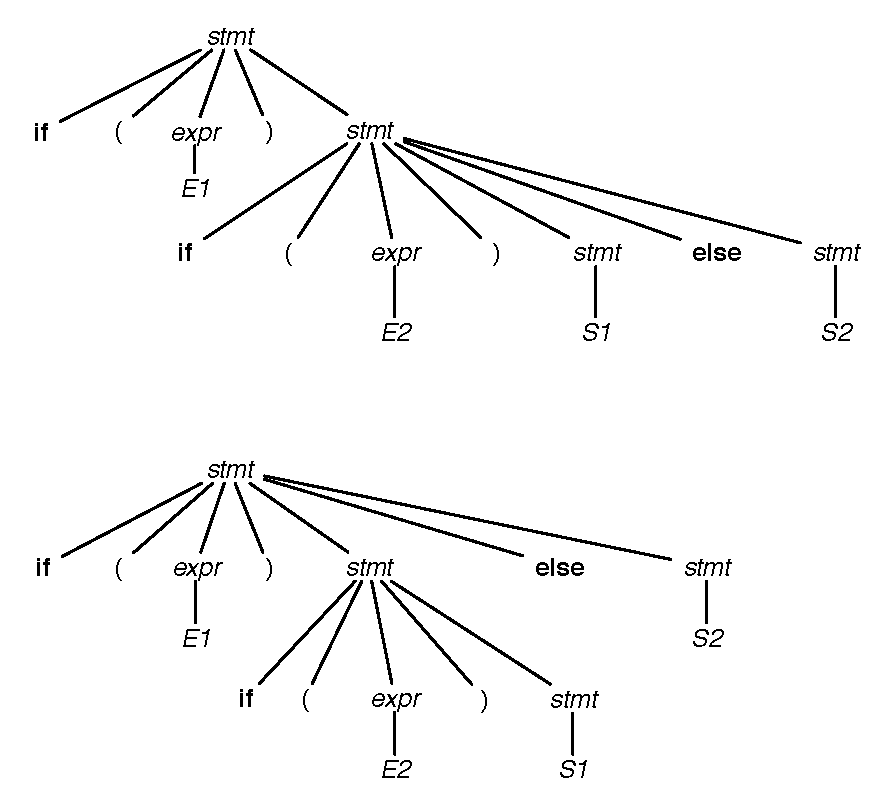
\includegraphics[scale=0.8]{figure/fig46.pdf}
 \end{center}
 \caption{曖昧な文法に対する2つの解析木}
 \label{fig:ambiguous_grammar}
\end{figure}

このような条件文の文法では普通、「各elseは前のほうにある未対応のthen文の
うち、もっとも近いものと対応する」という規則を設け、曖昧性を解消する。つ
まり図\ref{fig:ambiguous_grammar}の解析木のうち、上のほうを採用する。次の
ように文法を書き換えることで、曖昧さが解消できる。

\begin{align*}
 stmt & \rightarrow matched\_stmt \\
      & \quad\mid        unmatched\_stmt \\
 matched\_stmt & \rightarrow {\bf if}\ (expr)\ matched\_stmt\ {\bf
  else}\ matched\_stmt \\
      & \quad\mid S_1 \mid S_2 \mid S_3 \\
 unmatched\_stmt & \rightarrow {\bf if}\ (expr)\ stmt \\
                 & \quad\mid        {\bf if}\ (expr)\ matched\_stmt\ {\bf
		  else}\ unmatched\_stmt \\
 expr & \rightarrow E_1 \mid E_2
\end{align*}

\section{左再帰}
\label{121145_31Mar06}

$A \stackrel{*}{\Rightarrow} A\alpha$という導出が存在するとき、この文法は
{\bfseries 左再帰}であるという。後述するが、左再帰の文法は構文解析では扱
いがやっかいである。特に本講義で述べる手法では、構文解析が停止しない状況
が起こってしまう。

幸い、左再帰文法は、それと等価(同じ言語を生成する)で左再帰を含まない文
法に必ず変形することができる。ここでは、$A \rightarrow A\alpha$という形の
生成規則を持つ左再帰文法を、左再帰ではない文法に変換する方法のみ示す。左
再帰の文法のA-生成規則は、一般に
\[
 A \rightarrow A\alpha_1 \mid A\alpha_2 \mid \cdots \mid A\alpha_m \mid \beta_1 \mid
 \beta_2 \mid \cdots \mid \beta_n
\]
と書ける。ここで$\beta_i$は$A$以外の記号で始まる記号列である。このとき、
このA-生成規則を次のように変形する。
\begin{eqnarray*}
 A & \rightarrow & \beta_1 A' \mid \beta_2 A' \mid \cdots \mid \beta_n A' \\
 A' & \rightarrow & \alpha_1 A' \mid \alpha_2 A' \mid \cdots \mid \alpha_m A' \mid \epsilon
\end{eqnarray*}
この文法は、変形前のものと同じ言語を生成し、かつ左再帰を含まない。

\section{文脈自由文法の限界}
\label{110128_3Apr06}

言語$L = \{wcw \mid w \in (a \mid b)^* \}$は「$c$の前後に同じ文字列$w$が
出現するような言語」であり、プログラミング言語での「変数を使うときには、
それより前に宣言をしておかなければならない」という決まりを抽象化したもの
と言える。ところが、実は$L$は文脈自由文法では表現できない。つまり、変数を
使う前に宣言されているか検査するのは、構文解析部では行うことができない。
実際、この検査は、意味解析部で行われている。

このように、プログラミング言語の制限には構文解析部で検査できないものがあ
り、それらは意味解析部で検査されることが多い。

\section*{練習問題}

\begin{exercise}
 \label{ex:cfg_03}
 次の文脈自由文法について、トークン列 8 - 2 + 6 の解析木を示せ。可能なす
 べての場合を示し、自然な式の意味になるものはどれか示せ。
 \[
  string \rightarrow string + string \mid string - string \mid 0 \mid 1
 \mid 2 \mid 3 \mid 4 \mid 5 \mid 6 \mid 7 \mid 8 \mid 9
 \]
\end{exercise}
\begin{exercise}
 文脈自由文法$S \rightarrow 0 S 1 \mid 0 1$はどのような言語を表すか述べよ。
 \label{ex:cfg_04}
\end{exercise}
\begin{exercise}
 次の文法を考える。
  \begin{eqnarray*}
   S & \rightarrow & A1B \\
   A & \rightarrow & 0A \mid \epsilon \\
   B & \rightarrow & 0B \mid 1B \mid \epsilon
  \end{eqnarray*}
 この文法に対し、文字列$00101$の最左導出、最右導出を示せ。
 \label{ex:cfg_01}
\end{exercise}
\begin{exercise}
 算術式に対する文法
  \begin{eqnarray*}
   E & \rightarrow & E + T \mid T \\
   T & \rightarrow & T * F \mid F \\
   F & \rightarrow & (E) \mid {\bf id}
  \end{eqnarray*}
 を、左再帰でないように変形せよ。
 \label{ex:cfg_02}
\end{exercise}
